\section{Avaliação experimental}

\plain{Avaliação Experimental}

\subsection{Testbed}

\begin{frame}
  \frametitle{Testbed}

  \begin{figure}
          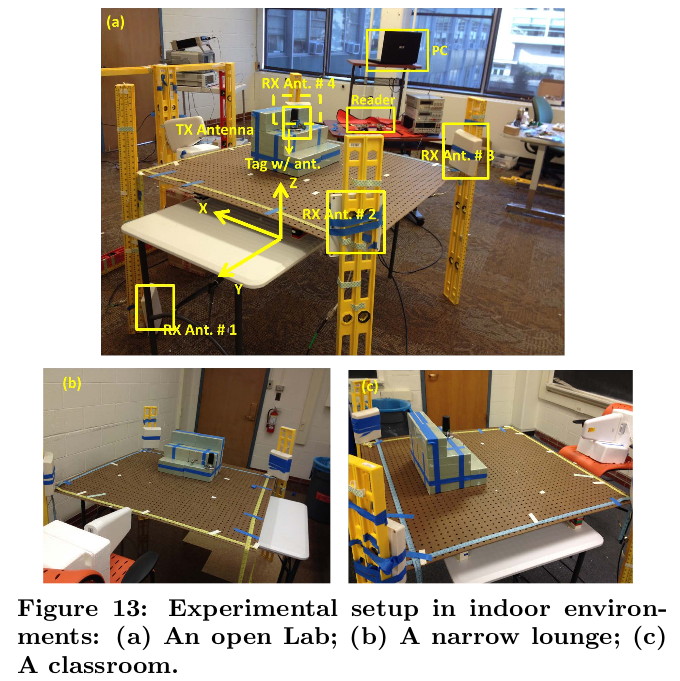
\includegraphics[scale=0.33]{testbed.png}
  \end{figure}
\end{frame}

\subsection{Experimentos}

\begin{frame}
  \frametitle{Medidas de Alcance 1D}

  \begin{figure}
          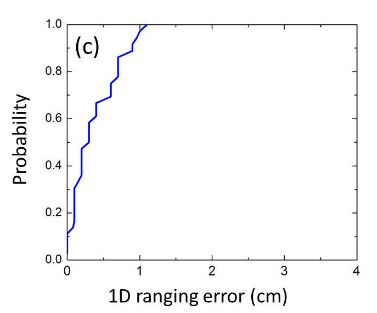
\includegraphics[width=6cm]{experiment_1D.png}
  \end{figure}
\end{frame}

\begin{frame}
  \frametitle{Medidas de Localização 2D}

  \begin{figure}
          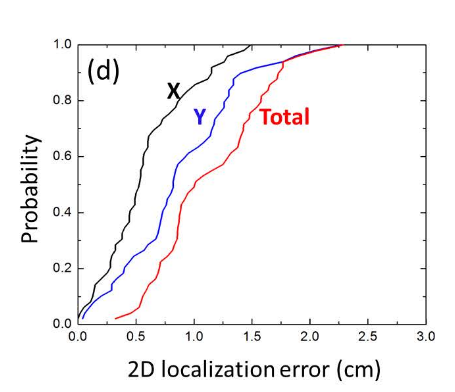
\includegraphics[width=5cm]{experiment_2D_probability.png}
          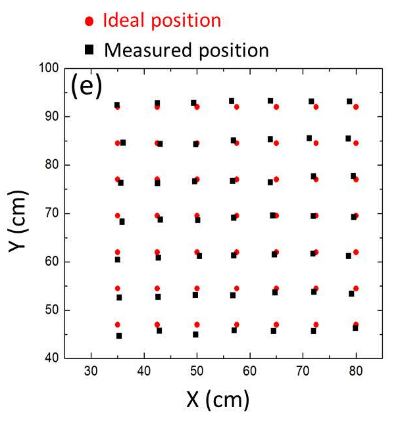
\includegraphics[width=5cm]{experiment_2D_position.png}
  \end{figure}
\end{frame}

\begin{frame}
  \frametitle{Medidas de Localização 3D}

  \begin{figure}
    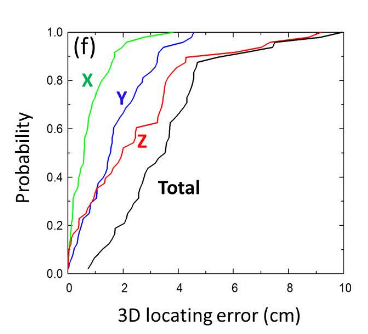
\includegraphics[width=4cm]{experiment_3D_in_open_lab.png}\hfil
    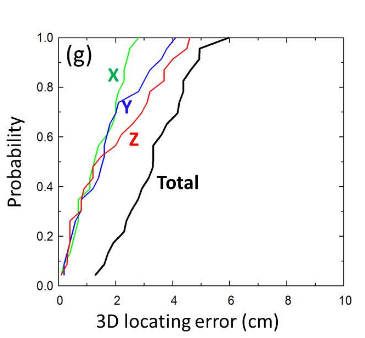
\includegraphics[width=4cm]{experiment_3D_in_narrow_lounge.png}\newline
    \hfil\hfil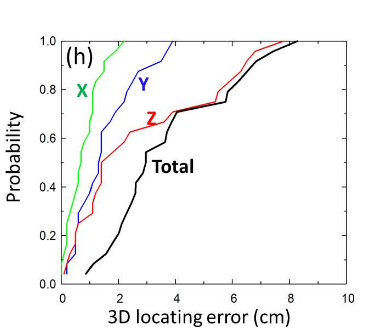
\includegraphics[width=4cm]{experiment_3D_in_classroom.png}
        \end{figure}
\end{frame}

\begin{frame}
  \frametitle{Localização com Elementos de Dispersão}

  \begin{figure}
          \centering
    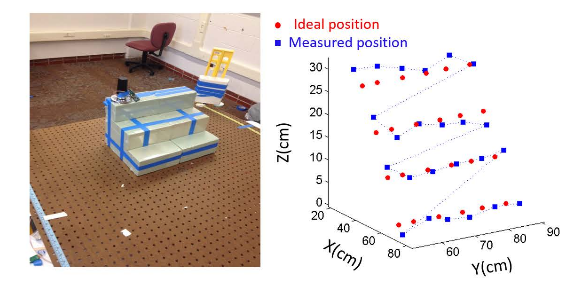
\includegraphics[width=7cm]{experiment_3D_without_scatter.png}
                \vfill
    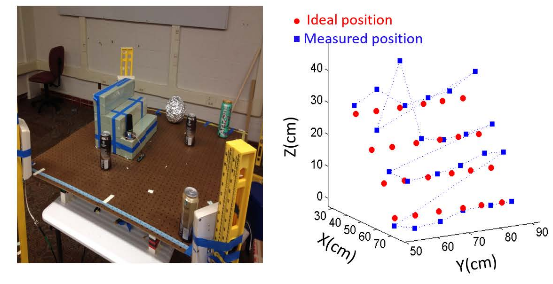
\includegraphics[width=7cm]{experiment_3D_with_5_scatters.png}
        \end{figure}
\end{frame}

\begin{frame}
  \frametitle{Localização com Elementos de Dispersão}

  \begin{figure}
          \vfill
          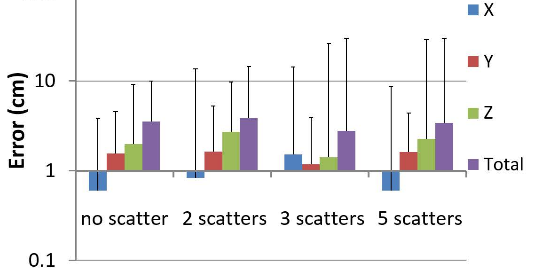
\includegraphics[width=9cm]{experiment_3D_error.png}
  \end{figure}
\end{frame}

\begin{frame}
  \frametitle{Monitoramento 3D em Tempo Real}

  \begin{figure}
          \vfill
          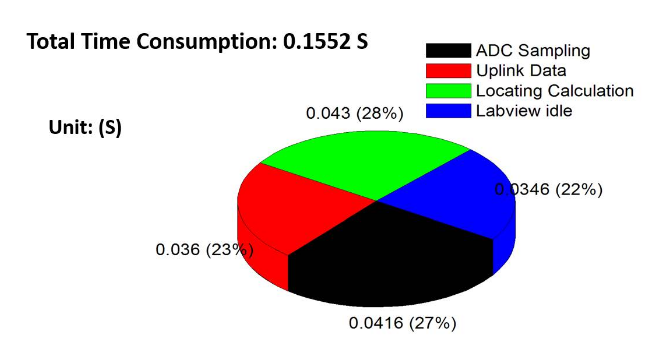
\includegraphics[width=9cm]{experiment_real_time_latency.png}
  \end{figure}
\end{frame}

\begin{frame}
  \frametitle{Vídeo de Apresentação}
    Vídeo de 1 minuto, no YouTube, sobre o artigo:
    \begin{itemize}
        \item \url{https://youtu.be/FwmQvAi7omo}
    \end{itemize}
\end{frame}

\section{Discussões}

\begin{frame}
  \frametitle{Discussões}

    \begin{itemize}
        \item Uso legítimo do espectro
            \begin{itemize}
                \item Legalidade na re-radiação harmônica
                \item Legalidade no leitor
            \end{itemize}
        \item Limitações no intervalo de leitura
        \item Custo da tecnologia
    \end{itemize}
\end{frame}

\section{Conclusão}

\begin{frame}
  \frametitle{Conclusão}

        \begin{itemize}
    \item Sistema de localização 3D em tempo real
                \begin{itemize}
      \item Erro médio de 3.5cm
                        \item Latência média de 0.155seg
                \end{itemize}
                \item Não necessita de nenhum movimento relativo ou nós de referência
        \end{itemize}
\end{frame}
